\documentclass[a4paper]{article}
\usepackage[utf8]{inputenc}
\usepackage[T1]{fontenc}
%\usepackage[french]{babel}
\usepackage{listings}
\usepackage{color}
\usepackage[usenames,dvipsnames,svgnames,table]{xcolor}
%\usepackage{titlesec}
\usepackage{tikz}
\usetikzlibrary{trees}
\usetikzlibrary{decorations.pathmorphing}
\usetikzlibrary{decorations.markings}


% Title Page
\title{SER - Labo1 \\ Sérialisation textuelle avec XML \& JSON}
\author{Yann Lederrey \& Joel Schär}


    \lstset{
    	tabsize=3,
    	inputencoding=utf8,
    	frame=lines,
    	caption=Test,
    	label=code:sample,
    	frame=shadowbox,
    	rulesepcolor=\color{gray},
    	xleftmargin=20pt,
    	framexleftmargin=15pt,
    	keywordstyle=\color{blue},
    	commentstyle=\color{OliveGreen},
    	stringstyle=\color{red},
    	numbers=left,
    	numberstyle=\scriptsize,
    	numbersep=5pt,
    	breaklines=true,
    	showstringspaces=false,
    	basicstyle=\footnotesize,
    	emph={cinema, projections, films, acteurs, motsCle, genres, langages, critiques },emphstyle={\color{magenta}}
    }
    
    \colorlet{punct}{red!60!black}
    \definecolor{delim}{RGB}{20,105,176}
    \colorlet{numb}{magenta!60!black}
    
    \lstdefinelanguage{json}{
    	stepnumber=1,
    	numbersep=5pt,
    	showstringspaces=false,
    	breaklines=true,
    	literate=
    	*{0}{{{\color{numb}0}}}{1}
    	{1}{{{\color{numb}1}}}{1}
    	{2}{{{\color{numb}2}}}{1}
    	{3}{{{\color{numb}3}}}{1}
    	{4}{{{\color{numb}4}}}{1}
    	{5}{{{\color{numb}5}}}{1}
    	{6}{{{\color{numb}6}}}{1}
    	{7}{{{\color{numb}7}}}{1}
    	{8}{{{\color{numb}8}}}{1}
    	{9}{{{\color{numb}9}}}{1}
    	{:}{{{\color{punct}{:}}}}{1}
    	{,}{{{\color{punct}{,}}}}{1}
    	{\{}{{{\color{delim}{\{}}}}{1}
    	{\}}{{{\color{delim}{\}}}}}{1}
    	{[}{{{\color{delim}{[}}}}{1}
    	{]}{{{\color{delim}{]}}}}{1},
    }
    
    
    \definecolor{amber}{rgb}{1.0, 0.49, 0.0}
    \definecolor{jaune}{rgb}{1.0, 0.75, 0.0}
    \definecolor{amethyst}{rgb}{0.6, 0.4, 0.8}
    \definecolor{antiquebrass}{rgb}{0.8, 0.58, 0.46}
    \definecolor{aqua}{rgb}{0.0, 1.0, 1.0}
    \definecolor{babypink}{rgb}{0.96, 0.76, 0.76}
   
   %delete first line indent
   \setlength{\parindent}{0in}
    
\begin{document}
\maketitle
\pagebreak

\tableofcontents
\pagebreak

\section{Introduction}
Ce rapport détail les mises en forme que nous avons choisie pour notre structure des documents XML et JSON. Nous illustrons notamment cette structure sous forme d'arbre avec un choix de couleurs différenciant chaque type d'élément.

\section{XML}
Pour la construction de notre DTD ainsi que notre template de fichier XML nous nous sommes basé sur la partie ``objectif'' du document de laboratoire ainsi que le schéma de base de données pour connaitre les cardinalités.\\
Dans l'écriture de notre fichier nous avons privilégié l'utilisation des balises en lieu et place des attributs. La raison est que pour nous la lecture du document nous parait plus simple si nous privilégions les balises. Le parsing de nos fichiers et leur créations nous paraissent aussi plus simple si 
nous utilisons des balises.\\
\\
Afin d'éviter de trop longs fichiers avec une balises générale ``projection'' reprenant ensuite tous les attributs à l'intérieur nous avons choisi d'utiliser des ``ID'' en séparant alors en bloc XML nos différents ``objets''.
\subsection{Graph XML}
\tikzset{
	photon/.style={decorate, decoration={snake}, draw=green},
	normal/.style={draw=black}
}
\subsubsection{Explication graphiques}
Chaque Noeud cinema correspond au noeud parent du fichier XML.\\
Les noeuds bleu correspondent aux éléments.\\
Les noeuds verts correspondent à des attributs.\\
Les noeuds colorés correspondent à des Id (ID et FK liés selon la couleur).

\begin{center}
	\begin{tikzpicture}[
	attribut/.style={rectangle,draw,fill=green!20},
	normal/.style={rectangle,draw,fill=blue!20,rounded corners=.8ex},
	filmid/.style={rectangle,draw,fill=amber!50,rounded corners=.8ex},
	acteurid/.style={rectangle,draw,fill=jaune!50,rounded corners=.8ex},
	genreid/.style={rectangle,draw,fill=amethyst!50,rounded corners=.8ex},
	critiqueid/.style={rectangle,draw,fill=antiquebrass!50,rounded corners=.8ex},
	motcleid/.style={rectangle,draw,fill=aqua!50,rounded corners=.8ex},
	langageid/.style={rectangle,draw,fill=babypink!50,rounded corners=.8ex},
	root/.style={rectangle,draw,fill=red!20},
	transform canvas={scale=0.8},
	sibling distance=7em,]
	\node [root]{cinema}
	child {node[normal] {projections} [normal]
		child { node[normal] {projection} [normal]
			child { node[normal] {dateProjection} [normal]}
			child { node[normal] {numeroSalle} [normal]}
			child { node[normal] {filmProj} [normal]
				child { node[filmid] {filmId} [normal]}
			}
			child { node[normal] {acteursProj} [normal]
				child { node[acteurid] {acteurProj} [normal]
					child { node[attribut] {acteurProjId} [normal]}
					child { node[attribut] {nomRole} [normal]}
					child { node[attribut] {placeRole} [normal]}
				}
			}
		}
	};
	\end{tikzpicture}
\end{center}

\newpage

\begin{center}
	\begin{tikzpicture}[
	attribut/.style={rectangle,draw,fill=green!20},
	normal/.style={rectangle,draw,fill=blue!20,rounded corners=.8ex},
	filmid/.style={rectangle,draw,fill=amber!50,rounded corners=.8ex},
	acteurid/.style={rectangle,draw,fill=jaune!50,rounded corners=.8ex},
	genreid/.style={rectangle,draw,fill=amethyst!50,rounded corners=.8ex},
	critiqueid/.style={rectangle,draw,fill=antiquebrass!50,rounded corners=.8ex},
	motcleid/.style={rectangle,draw,fill=aqua!50,rounded corners=.8ex},
	langageid/.style={rectangle,draw,fill=babypink!50,rounded corners=.8ex},
	root/.style={rectangle,draw,fill=red!20},
	transform canvas={scale=0.8},
	sibling distance=7em,]
	\node [root]{cinema}
	child {node[normal] {films} [normal]
		child { node[normal] {film} [normal]
			child { node[filmid] {filmId} [normal]}
			child { node[normal] {titre} [normal]}
			child { node[normal] {synopsis} [normal]}
			child { node[normal] {duree} [normal]}
			child { node[normal] {critiqueFilm} [normal]
				child { node[critiqueid] {critiquesFilmId} [normal]}
			}
			child { node[normal] {genresFilm} [normal]
				child { node[normal] {genreFilm} [normal]
					child { node[genreid] {genreFilmId} [normal]}
				}
			}
			child { node[normal] {motsCleFilm} [normal]
				child { node[normal] {motCleFilm} [normal]
					child { node[motcleid] {motCleFilmId} [normal]}
				}
			}
			child { node[normal] {langagesFilm} [normal]
				child { node[normal] {langageFilm} [normal]
					child { node[langageid] {langageFilmId} [normal]}
				}
			}
			child { node[normal] {photo} [normal]}
		}
	};
	\end{tikzpicture}
\end{center}

\vspace{170px}

\begin{center}
	\begin{tikzpicture}[
	attribut/.style={rectangle,draw,fill=green!20},
	normal/.style={rectangle,draw,fill=blue!20,rounded corners=.8ex},
	filmid/.style={rectangle,draw,fill=amber!50,rounded corners=.8ex},
	acteurid/.style={rectangle,draw,fill=jaune!50,rounded corners=.8ex},
	genreid/.style={rectangle,draw,fill=amethyst!50,rounded corners=.8ex},
	critiqueid/.style={rectangle,draw,fill=antiquebrass!50,rounded corners=.8ex},
	motcleid/.style={rectangle,draw,fill=aqua!50,rounded corners=.8ex},
	langageid/.style={rectangle,draw,fill=babypink!50,rounded corners=.8ex},
	root/.style={rectangle,draw,fill=red!20},
	transform canvas={scale=0.8},
	sibling distance=7em,]
	\node [root]{cinema}
	child { node[normal] {acteurs} [normal]
		child { node[normal] {acteur} [normal]
			child { node[acteurid] {acteurId} [normal]}
			child { node[normal] {nom} [normal]}
			child { node[normal] {nomNaissance} [normal]}
			child { node[normal] {biographie} [normal]}
			child { node[normal] {sexe} [normal]
				child { node[attribut] {type(enum)} [normal]}
			}
			child { node[normal] {dateNaissance} [normal]}
			child { node[normal] {dateDeces} [normal]}
		}
	};
	\end{tikzpicture}
\end{center}

\vspace{170px}

\begin{center}
	\begin{tikzpicture}[
	attribut/.style={rectangle,draw,fill=green!20},
	normal/.style={rectangle,draw,fill=blue!20,rounded corners=.8ex},
	filmid/.style={rectangle,draw,fill=amber!50,rounded corners=.8ex},
	acteurid/.style={rectangle,draw,fill=jaune!50,rounded corners=.8ex},
	genreid/.style={rectangle,draw,fill=amethyst!50,rounded corners=.8ex},
	critiqueid/.style={rectangle,draw,fill=antiquebrass!50,rounded corners=.8ex},
	motcleid/.style={rectangle,draw,fill=aqua!50,rounded corners=.8ex},
	langageid/.style={rectangle,draw,fill=babypink!50,rounded corners=.8ex},
	root/.style={rectangle,draw,fill=red!20},
	transform canvas={scale=0.8},
	level 1/.style={sibling distance=6cm},
	level 2/.style={sibling distance=3cm}, 
	level 3/.style={sibling distance=2cm},]
	\node [root]{cinema}
	child { node[normal] {motsCleFilm} [normal]
		child { node[normal] {motCle} [normal]
			child { node[motcleid] {motCleId} [normal]}
			child { node[normal] {labelMc} [normal]}
		}
	}
	child { node[normal] {genres} [normal]
		child { node[normal] {genre} [normal]
			child { node[genreid] {genreId} [normal]}
			child { node[normal] {labelGe} [normal]}
		}
	}
	child { node[normal] {langages} [normal]
		child { node[normal] {langage} [normal]
			child { node[langageid] {langageId} [normal]}
			child { node[normal] {labelLa} [normal]}
		}
	}
	child { node[normal] {critiques} [normal]
		child { node[normal] {critique} [normal]
			child { node[critiqueid] {critiqueId} [normal]}
			child { node[normal] {texte} [normal]}
			child { node[normal] {note} [normal]}
		}
	};
	\end{tikzpicture}
\end{center}

\vspace{170px}

\subsection{Fichier DTD}
\lstinputlisting[language=XML, caption={pathe.dtd}]{../pathe.dtd}
\subsection{Exemple XML}
\lstinputlisting[language=XML, caption={pathe.xml}]{../pathe.xml}
\subsection{Validation XML}
\lstinputlisting[language=json, caption={validation}]{../validation.txt}

\section{JSON}
Pour écrire notre template JSON, Nous n'avons pas fait de grands choix. Nous avons déterminé ``Projections'' comme un tableau de projection, ceux-ci étant des objets contenant un titre, une date ainsi qu'un objet ``Acteurs'' comprenant les deux roles.
\subsection{Graph JSON}

\begin{center}
	\begin{tikzpicture}[
	attribut/.style={rectangle,draw,fill=green!20},
	normal/.style={rectangle,draw,fill=blue!20,rounded corners=.8ex},
	filmid/.style={rectangle,draw,fill=amber!50,rounded corners=.8ex},
	acteurid/.style={rectangle,draw,fill=jaune!50,rounded corners=.8ex},
	genreid/.style={rectangle,draw,fill=amethyst!50,rounded corners=.8ex},
	critiqueid/.style={rectangle,draw,fill=antiquebrass!50,rounded corners=.8ex},
	motcleid/.style={rectangle,draw,fill=aqua!50,rounded corners=.8ex},
	langageid/.style={rectangle,draw,fill=babypink!50,rounded corners=.8ex},
	root/.style={rectangle,draw,fill=red!20},
	transform canvas={scale=0.8},
	sibling distance=7em,]
	\node [root]{cinema}
	child {node[normal] {projections} [normal]
		child { node[normal] {projection} [normal]
			child { node[normal] {TitreFilm} [normal]}
			child { node[normal] {DateProjection} [normal]}
			child { node[normal] {Acteurs} [normal]
				child { node[normal] {1er Role} [normal]}
				child { node[normal] {2eme Role} [normal]}
			}
		}
	};
	\end{tikzpicture}
\end{center}

\vspace{170px}

\subsection{Exemple JSON}
\lstinputlisting[language=json, caption={pathe.json}]{../pathe.json}

\section{conclusion}
Ce travail nous a permis de mieux comprendre la structure des formats XML et JSON. Nous avons expérimenter l'utilité d'avoir une grammaire DTD qui évite les inconsistances dans le document XML et permet de valider l'existence de tous les éléments. Nous n'avons pas rencontré de grand difficulté quand à la réalisation de ce travail.


\end{document}          
	